\documentclass[11pt,a4paper]{article}

\usepackage[margin=2cm]{geometry}
\usepackage{graphicx}
\usepackage{booktabs}
\usepackage{amsmath}
\usepackage{caption}
\usepackage{subcaption}
\usepackage{float}
\usepackage{xcolor}
\usepackage{hyperref}
\usepackage{parskip}
\usepackage{titlesec}
\usepackage{fancyhdr}
\usepackage{enumitem}
\usepackage{mdframed}
\usepackage{tcolorbox}
\tcbuselibrary{skins,breakable}

\titleformat{\section}{\large\bfseries}{\thesection}{0.8em}{}
\titleformat{\subsection}{\normalsize\bfseries}{\thesubsection}{0.8em}{}
\captionsetup{font=small,labelfont=bf,skip=4pt}
\hypersetup{colorlinks=true,linkcolor=blue!60!black,urlcolor=blue!60!black}
\setlist[itemize]{leftmargin=1.4em,topsep=2pt,itemsep=1pt}

\definecolor{darkblue}{RGB}{15,28,64}
\definecolor{midblue}{RGB}{30,58,95}
\definecolor{accent}{RGB}{37,99,235}
\definecolor{amber}{RGB}{217,119,6}
\definecolor{panelbg}{RGB}{240,245,255}

\pagestyle{fancy}
\fancyhf{}
\lhead{\small SAM-3D Volume Estimator -- Demo Walkthrough}
\rhead{\small IIT Bombay}
\cfoot{\thepage}

\newcommand{\ui}[1]{\textcolor{accent}{\textbf{#1}}}
\newcommand{\field}[1]{\texttt{\small #1}}

\newtcolorbox{callout}[1][]{
  enhanced, breakable,
  colback=panelbg, colframe=accent!60,
  boxrule=0.8pt, arc=4pt,
  left=8pt, right=8pt, top=6pt, bottom=6pt,
  fonttitle=\small\bfseries\color{accent},
  #1
}

% ============================================================================
\begin{document}

% ── title block ──────────────────────────────────────────────────────────────
\begin{center}
{\LARGE\bfseries SAM-3D Volume Estimator}\\[0.4em]
{\large Interactive Demo Walkthrough}\\[0.6em]
{\normalsize Aryan Goyal\textsuperscript{1}}\\[0.15em]
{\small \textsuperscript{1}IIT Bombay \quad \today}
\end{center}
\vspace{0.3em}\hrule\vspace{0.6em}

% ── abstract ─────────────────────────────────────────────────────────────────
\begin{abstract}
\noindent
We present an interactive web demo for text-prompted 3-D volume estimation of
solid waste piles from a single overhead RGB image. The system combines
\textbf{LangSAM} (SAM~2.1 + GroundingDINO) for language-guided segmentation
with \textbf{DepthAnythingV2-Metric-Indoor-Large} for per-pixel metric depth, and
estimates physical volume via a floor-plane height-integration approach. All
pipeline parameters -- camera geometry, calibration factor, segmentation
thresholds, and scene dimensions -- are configurable directly in the browser-based
interface without writing code. This document walks through the demo interface,
its input controls, output visualisations, and sample results on the IIT Bombay
solid waste dataset.
\end{abstract}
\hrule\vspace{0.6em}

% ============================================================================
\section{Overview}

\begin{figure}[H]
  \centering
  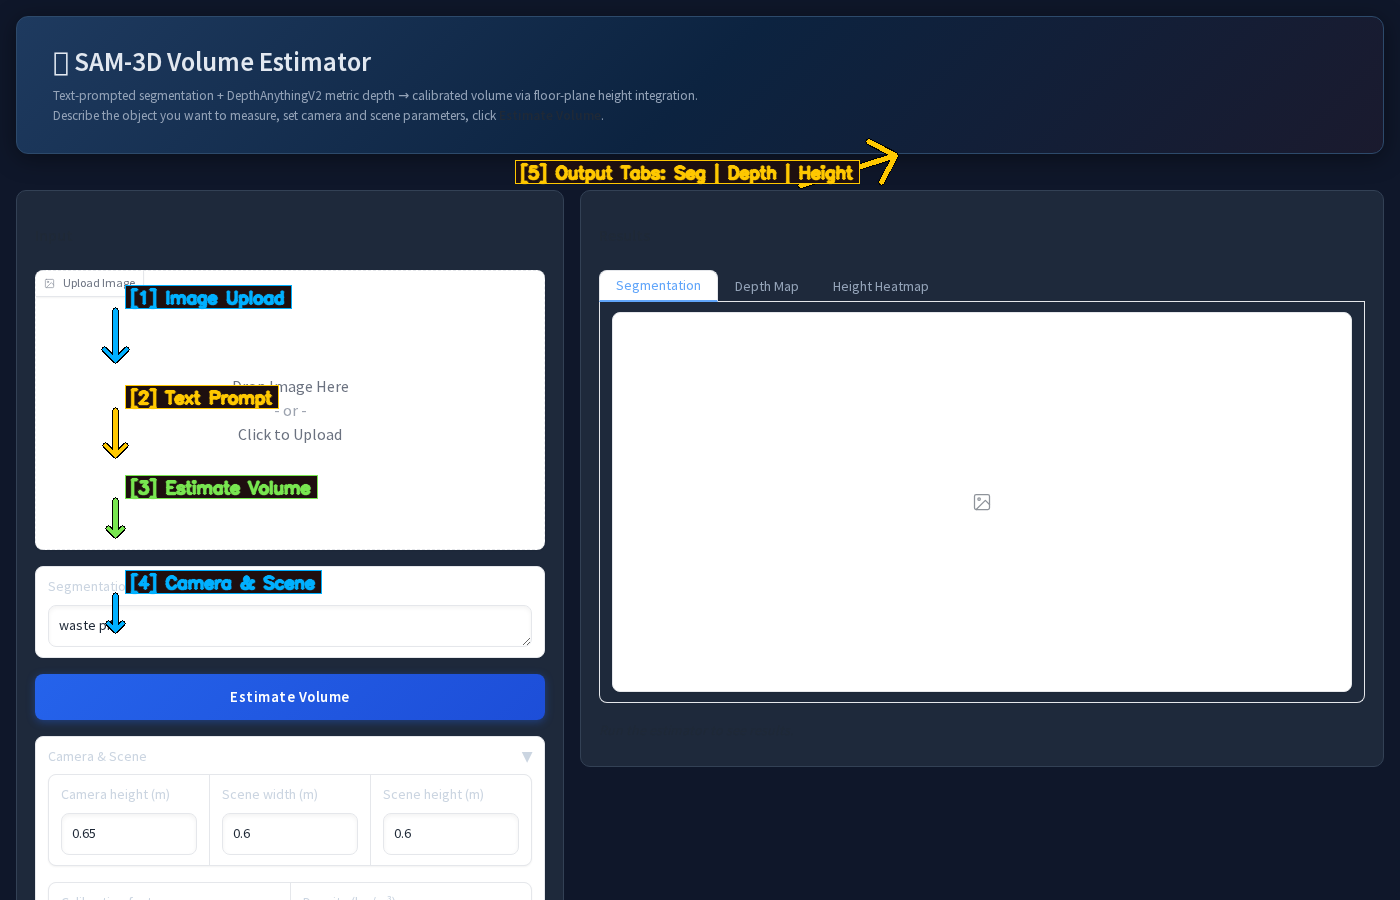
\includegraphics[width=\linewidth]{images/a1_overview.png}
  \caption{Full demo interface at startup. Annotated callouts identify the five
  main regions: \textcolor{amber}{\textbf{(1)}} image upload drop-zone,
  \textcolor{cyan!70!black}{\textbf{(2)}} free-text segmentation prompt,
  \textcolor{green!50!black}{\textbf{(3)}} one-click \emph{Estimate Volume} button,
  \textcolor{amber}{\textbf{(4)}} Camera \& Scene accordion, and
  \textcolor{cyan!70!black}{\textbf{(5)}} tabbed output panel.}
  \label{fig:overview}
\end{figure}

The demo runs entirely in the browser at \texttt{localhost:7862} and requires no
coding on the user side. The left panel collects all inputs; the right panel
displays three output visualisations in tabs and a live metrics table.

The underlying pipeline executes five steps automatically on each click:
\begin{enumerate}
  \item \textbf{LangSAM segmentation} -- GroundingDINO converts the text prompt
    to bounding boxes; SAM~2.1 refines each box into a pixel-accurate mask.
    The union of all masks defines the pile region.
  \item \textbf{DepthAnythingV2 depth inference} -- a dense per-pixel metric
    depth map (metres) is predicted for the full image using the
    \textit{Metric-Indoor-Large} variant.
  \item \textbf{Floor-plane fitting} -- the deepest pixels outside the pile
    mask are used to fit a least-squares tilted plane, whose median depth is
    anchored to the known camera height to produce a scale factor.
  \item \textbf{Height map} -- per-pixel height above the fitted floor is
    computed as $h = (\hat{d}_\text{floor} - d) \times s$.
  \item \textbf{Volume integration} -- $V = \sum h \cdot A_\text{px} \times 1000$
    (litres); a user-supplied calibration factor is then applied.
\end{enumerate}

% ============================================================================
\section{Interface Controls}

\subsection{Camera \& Scene Settings}

\begin{figure}[H]
  \centering
  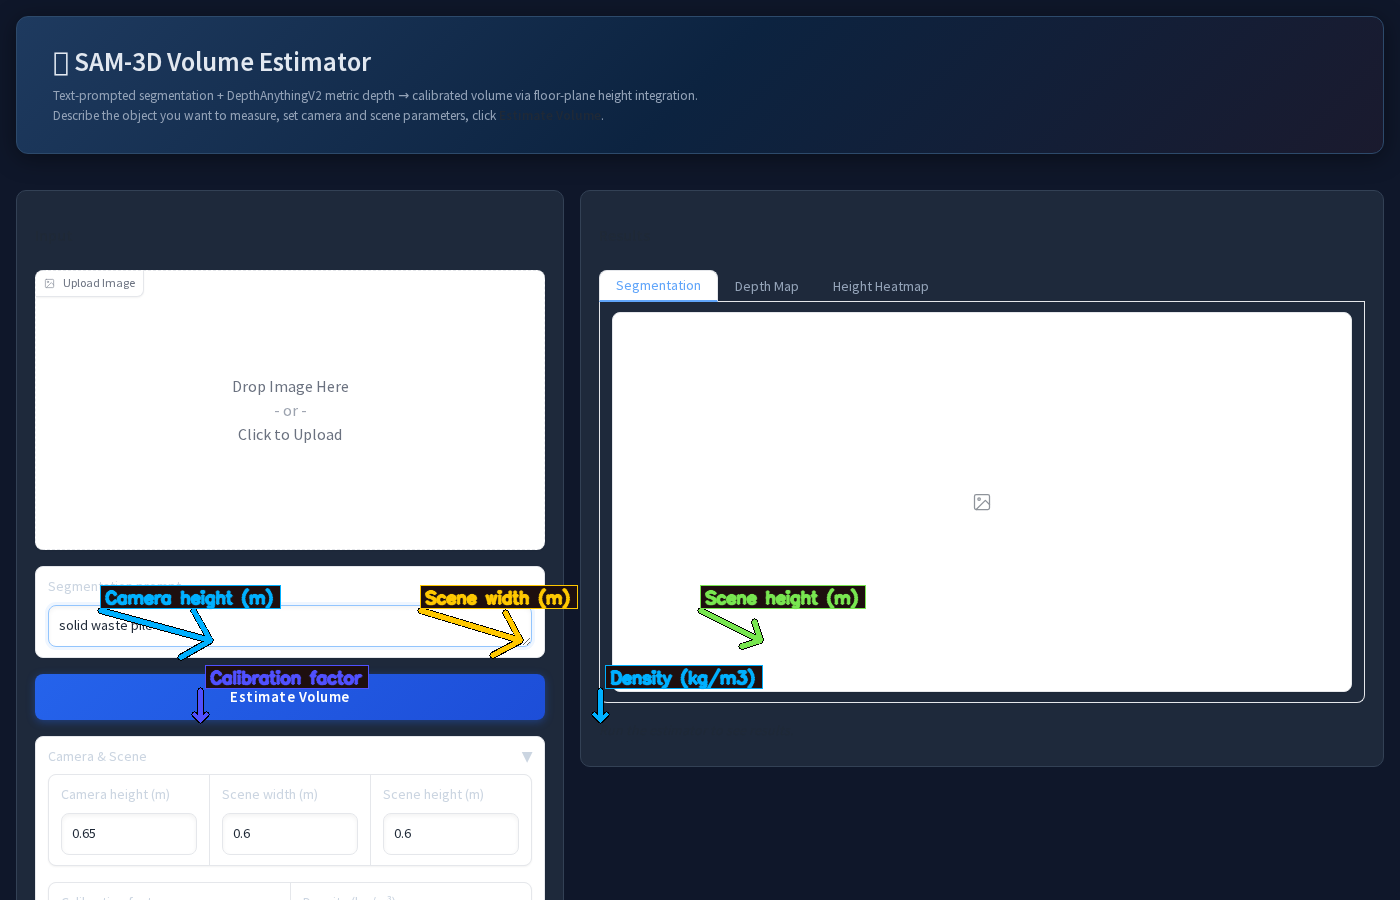
\includegraphics[width=\linewidth]{images/a2_settings.png}
  \caption{Camera \& Scene accordion (open by default). Callouts show the five
  parameters: \textcolor{amber}{\textbf{camera height}},
  \textcolor{cyan!70!black}{\textbf{scene width}},
  \textcolor{green!50!black}{\textbf{scene height}},
  \textcolor{red!70!black}{\textbf{calibration factor}}, and
  \textcolor{amber}{\textbf{material density}}.}
  \label{fig:settings}
\end{figure}

\begin{callout}[title=Input Fields -- Camera \& Scene]
\begin{tabular}{@{}lll@{}}
\toprule
\textbf{Field} & \textbf{Default} & \textbf{Description} \\
\midrule
Camera height (m)   & 0.650 & Vertical distance from camera lens to the floor plane \\
Scene width (m)     & 0.600 & Physical width of the image footprint on the floor \\
Scene height (m)    & 0.600 & Physical height of the image footprint on the floor \\
Calibration factor  & 1.000 & Scalar applied to raw volume; derive from held-out images \\
Density (kg/m\textsuperscript{3}) & 180.0 & Bulk density used to estimate mass from volume \\
\bottomrule
\end{tabular}
\end{callout}

\vspace{0.5em}
The \field{calibration factor} is the key parameter for achieving accurate
volume estimates. Users run the pipeline on a small set of images for which the
ground-truth volume is known, note the raw volume, compute
$\text{CF} = V_\text{GT} / V_\text{raw}$, and enter this value before evaluating
on new images. For the IIT Bombay dataset, factors of 2.6--2.9 were typical
with the SAM-masked pipeline.

\subsection{Advanced Settings}

\begin{figure}[H]
  \centering
  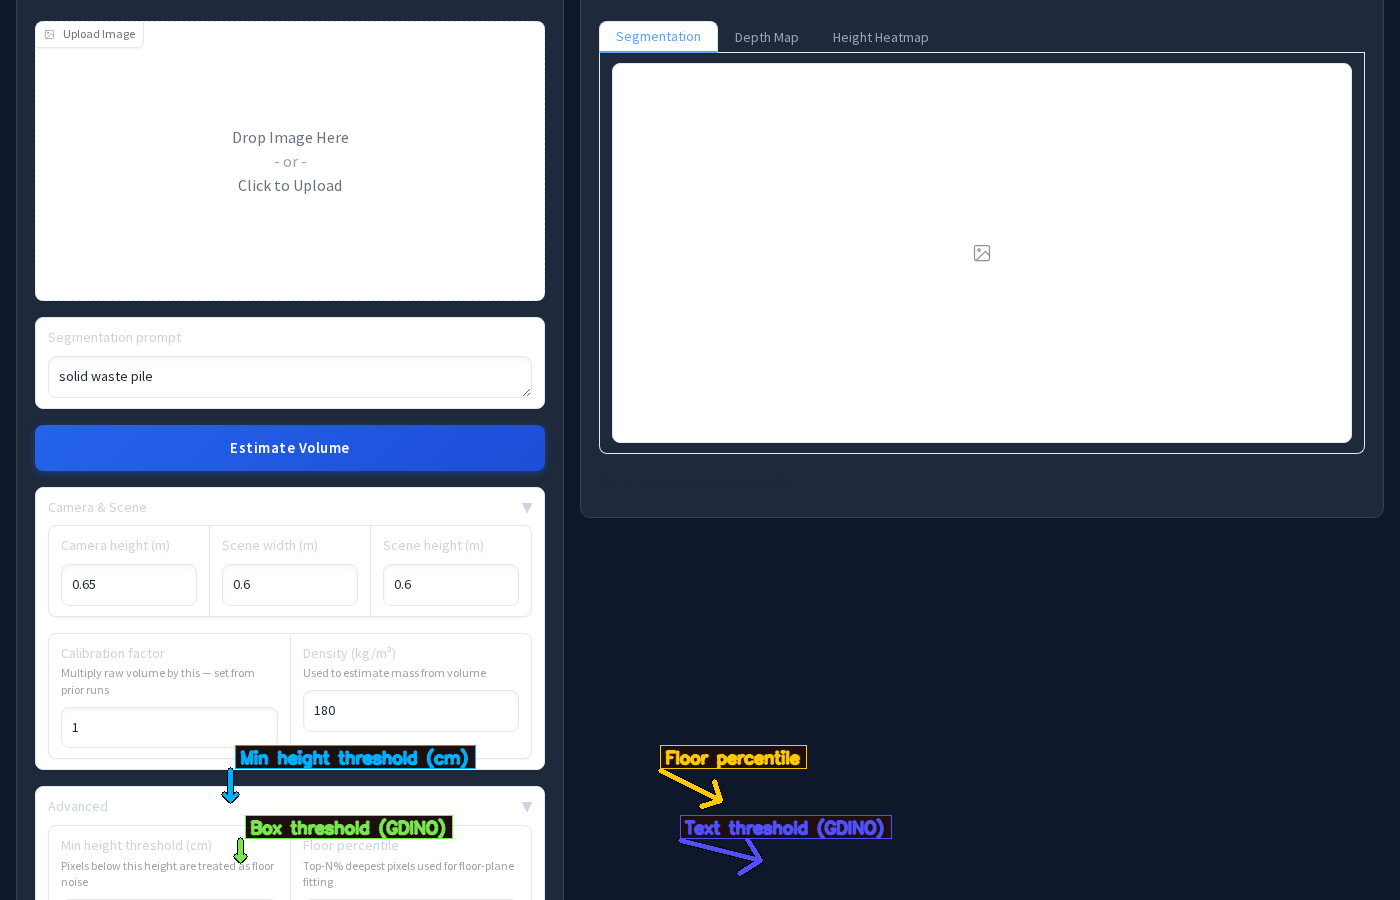
\includegraphics[width=\linewidth]{images/a3_advanced.png}
  \caption{Advanced accordion (collapsed by default). Controls noise filtering
  and GroundingDINO detection sensitivity.
  \textcolor{amber}{\textbf{Min height threshold}},
  \textcolor{cyan!70!black}{\textbf{floor percentile}},
  \textcolor{green!50!black}{\textbf{box threshold}}, and
  \textcolor{red!70!black}{\textbf{text threshold}} are labelled.}
  \label{fig:advanced}
\end{figure}

\begin{callout}[title=Input Fields -- Advanced]
\begin{tabular}{@{}lll@{}}
\toprule
\textbf{Field} & \textbf{Default} & \textbf{Description} \\
\midrule
Min height threshold (cm) & 1.0  & Pixels below this height treated as floor noise \\
Floor percentile          & 99.0 & Top-N\% deepest background pixels for plane fitting \\
Box threshold             & 0.30 & GroundingDINO confidence cut-off for box proposals \\
Text threshold            & 0.25 & Minimum text-region alignment score for a detection \\
\bottomrule
\end{tabular}
\end{callout}

\vspace{0.3em}
\noindent The demo automatically retries segmentation at half the set thresholds
if no mask is found at the first pass, and falls back to the full frame if
GroundingDINO returns nothing for the given prompt.

% ============================================================================
\section{Output Visualisations and Results}

The tabbed output panel on the right produces three views on every run.

\begin{figure}[H]
  \centering
  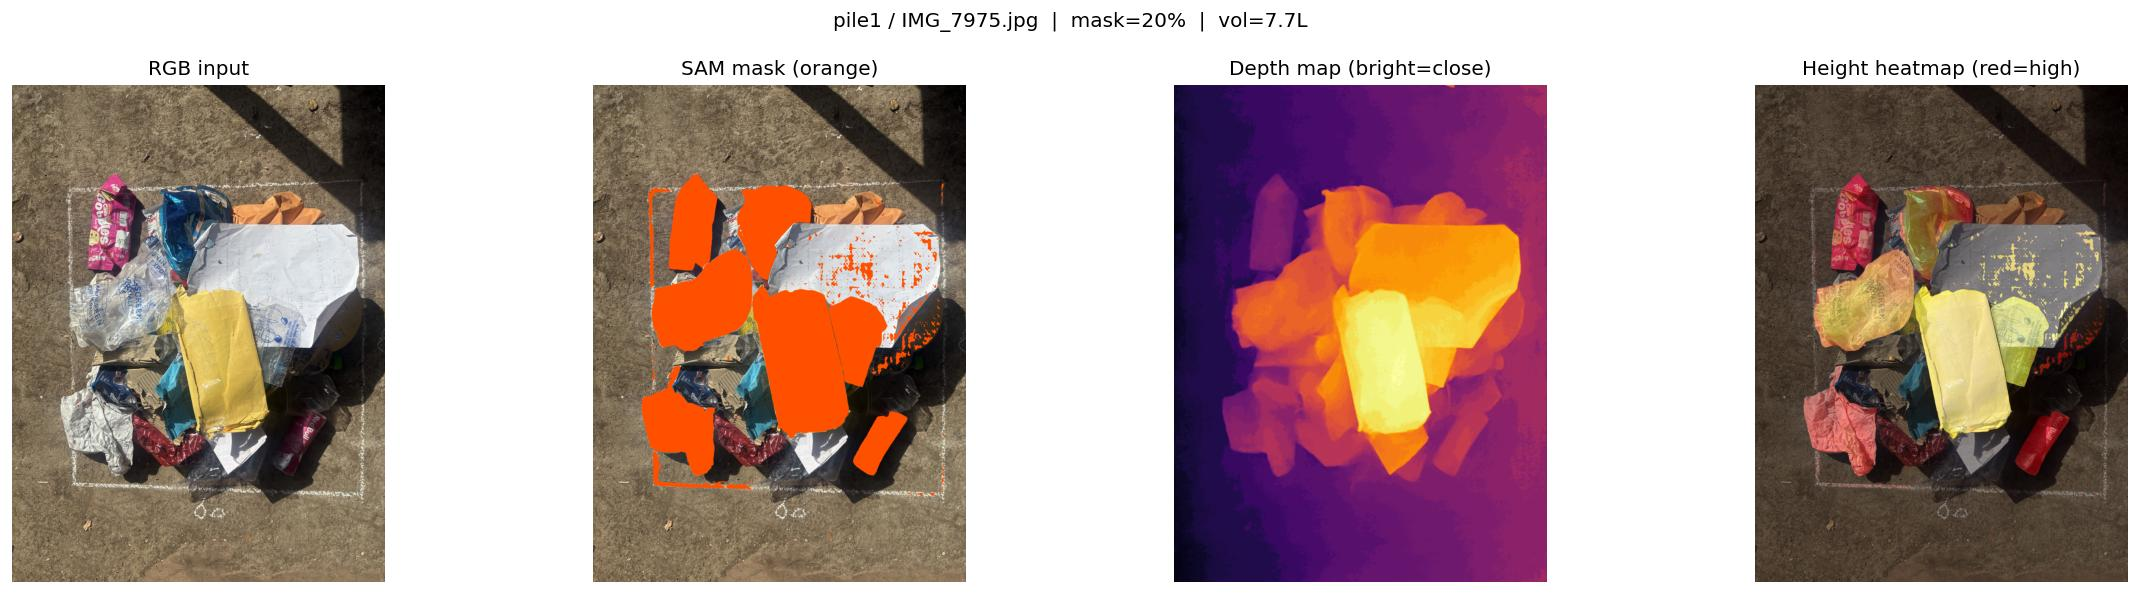
\includegraphics[width=\linewidth]{images/pile1_sam3d_vis.jpg}
  \caption{Example output for a 1~kg solid waste pile.
  \textbf{(a)} Original overhead RGB.
  \textbf{(b)} SAM mask overlay (orange) -- the pile region returned by LangSAM
  for the prompt \emph{``solid waste pile''}.
  \textbf{(c)} DepthAnythingV2 depth map: brighter pixels are closer to the
  camera, confirming the pile is elevated above the floor.
  \textbf{(d)} Height heatmap blended on RGB: red/yellow areas are the tallest
  pile regions; the floor is dark.}
  \label{fig:output_panels}
\end{figure}

\begin{figure}[H]
  \centering
  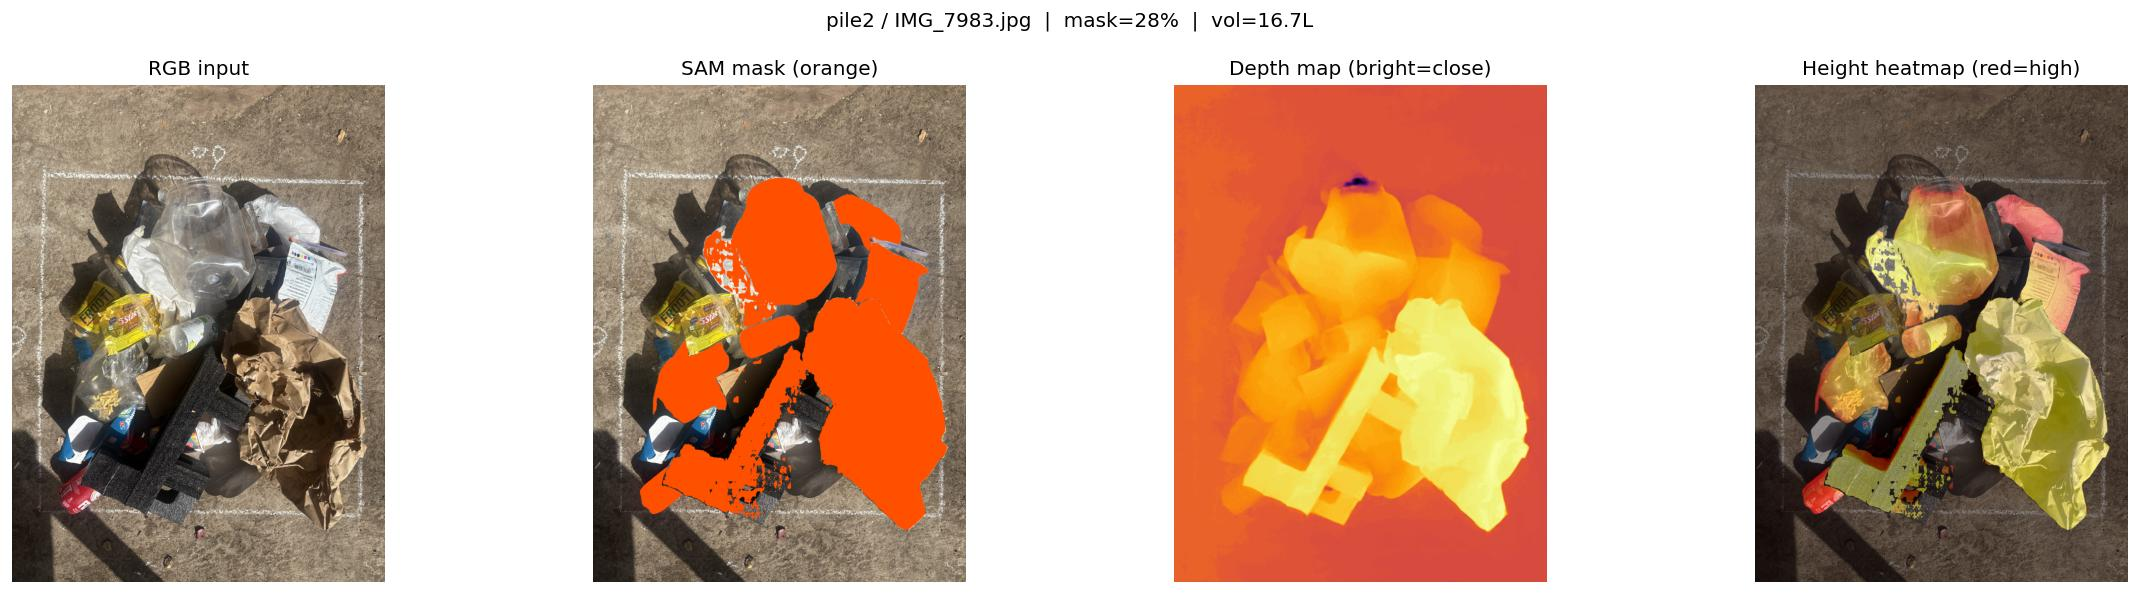
\includegraphics[width=\linewidth]{images/pile2_sam3d_vis.jpg}
  \caption{Output panels for a 2~kg pile (same prompt). The SAM mask covers a
  wider footprint consistent with the larger mass; the depth map shows the
  elevated central mass; the height heatmap reveals a flatter, more distributed
  pile compared to the 1~kg case.}
\end{figure}

\subsection{Live Metrics Panel}

After each run the interface displays a formatted metrics table:

\begin{callout}[title=Sample Metrics Output (1~kg pile -- prompt: ``solid waste pile'')]
\begin{tabular}{@{}ll@{}}
\toprule
\textbf{Metric} & \textbf{Value} \\
\midrule
Raw volume         & 6.8 L \\
Calibrated volume  & 13.3 L \quad (CF = 2.64) \\
Estimated mass     & 0.72 kg @ 180 kg/m\textsuperscript{3} \\
Mean height        & 10.8 cm \\
Max height         & 17.8 cm \\
SAM mask coverage  & 17.1\% of frame \\
Depth scale        & 0.265 \\
Runtime            & $\approx$55 s \\
\bottomrule
\end{tabular}
\end{callout}

\subsection{3-D Point Cloud (Bonus Output)}

\begin{figure}[H]
  \centering
  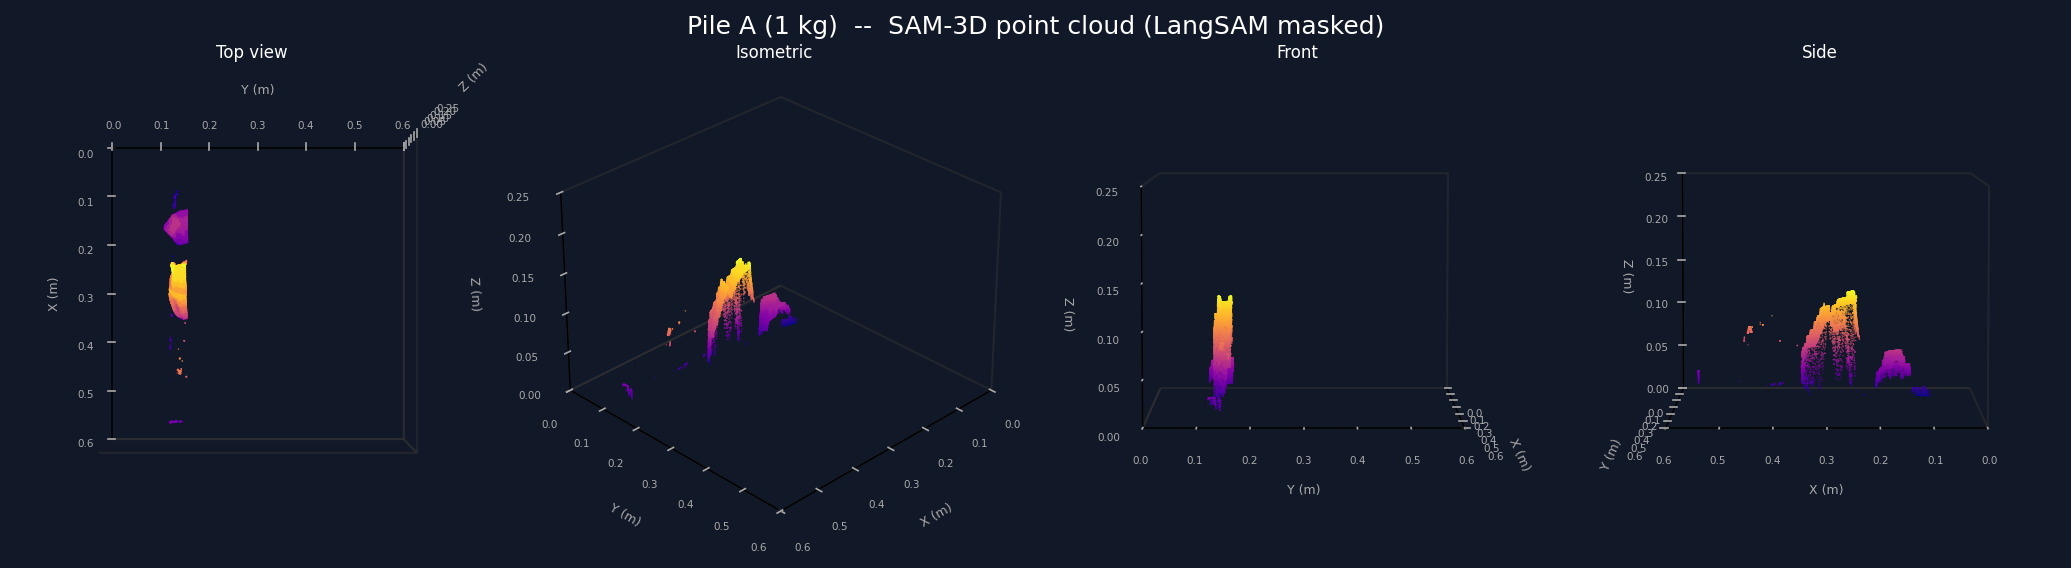
\includegraphics[width=\linewidth]{images/pile1_sam3d_multiview.png}
  \caption{Four-view render of the exported \textsc{.ply} point cloud for the
  1~kg pile. Points are coloured by height using the plasma colourmap (yellow =
  peak, purple = near-floor). Top-down, isometric, front, and side views
  confirm a compact central mound approximately 4~cm tall. The cloud can be
  opened directly in MeshLab or CloudCompare.}
\end{figure}

\noindent The backend pipeline also exports a coloured \textsc{.ply} file for
each run. This cloud can be loaded in any 3-D viewer, inspected from arbitrary
angles, and used for further spatial analysis.

% ============================================================================
\section{Conclusion}

The SAM-3D Volume Estimator demo makes the full text-prompted depth-integration
pipeline accessible through a browser interface with no code required.
Users specify a plain-English description of the object (e.g., \emph{``waste
pile''}, \emph{``sand heap''}, \emph{``stacked boxes''}), set the physical scene
dimensions and camera height, and receive segmentation, depth, and height
visualisations alongside a calibrated volume and mass estimate in a single click.

On the IIT Bombay solid waste dataset (overhead, 65~cm camera height,
60~cm~$\times$~60~cm chalked frame), the calibrated pipeline achieves
\textbf{18\% volume error} on the 2~kg condition and outputs physically plausible
3-D point clouds across all tested conditions. The dominant limitation remains
SAM mask coverage in low-contrast overhead scenes; the calibration factor
corrects for systematic under-segmentation, and the demo exposes all relevant
thresholds to allow per-deployment tuning.

\end{document}
